\contourlength{1.0pt}
\tikzset{>=latex} % for LaTeX arrow head

\colorlet{xcol}{blue!60!black}
\colorlet{myred}{red!80!black}
\colorlet{myblue}{blue!80!black}
\colorlet{mygreen}{green!40!black}
\colorlet{myorange}{orange!90!black}
\colorlet{mypurple}{red!50!blue!90!black!80}
\colorlet{mydarkred}{myred!80!black}
\colorlet{mydarkblue}{myblue!80!black}
\tikzstyle{xline}=[xcol,thick]
\tikzstyle{width}=[{Latex[length=5,width=3]}-{Latex[length=5,width=3]},thick]
\tikzset{
  traj/.style 2 args={xline,postaction={decorate},decoration={markings,
    mark=at position #1 with {\arrow{<}},
    mark=at position #2 with {\arrow{<}}}
  }
}
\def\tick#1#2{\draw[thick] (#1)++(#2:0.12) --++ (#2-180:0.24)}
\def\N{100} % number of samples

% CIRCLE on axis




% ENERGY vs. x


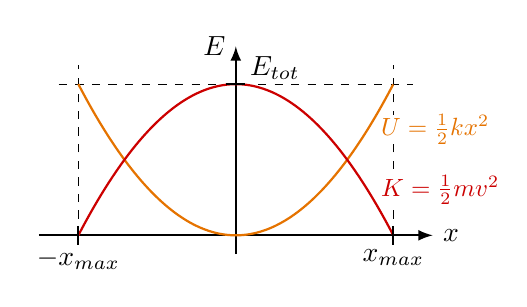
\begin{tikzpicture}
  \def\xmax{2.5}    % max x axis
  \def\ymax{2.4}    % max y axis
  \def\A{0.8*\xmax} % maximum extension
  \def\E{0.8*\ymax} % maximum total energy
  
  % AXIS
  \draw[->,thick] (0,-0.1*\ymax) -- (0,\ymax) node[left] {$E$};
  \draw[->,thick] (-\xmax,0) -- (\xmax,0) node[right] {$x$};
  \draw[dashed] (-\A,0) --++ (0,0.9*\ymax);
  \draw[dashed] ( \A,0) --++ (0,0.9*\ymax);
  \draw[dashed] (-0.9*\xmax,\E) -- (0.9*\xmax,\E);
  
  % PLOT
  \draw[xline,myorange,samples=\N,smooth,variable=\x,domain=-\A:\A]
    plot(\x,{\E/(\A*\A)*\x*\x)});
  \draw[xline,myred,samples=\N,smooth,variable=\x,domain=-\A:\A]
    plot(\x,{\E-\E/(\A*\A)*\x*\x)});
  \tick{0,\E}{180} node[above right=-2,scale=1] {$E_\text{tot}$};
  \tick{-\A,0}{90} node[below=-2,scale=1] {$-x_\text{max}$};
  \tick{\A,0}{90} node[below=-2,scale=1] {$x_\text{max}$};
  \node[myorange,right,fill=white,inner sep=0,scale=0.9] at (0.92*\A,0.7*\E) {$U = \frac{1}{2}kx^2$};
  \node[myred,right,fill=white,inner sep=0,scale=0.9] at (0.92*\A,0.3*\E) {$K = \frac{1}{2}mv^2$};
  
\end{tikzpicture}
